\documentclass[14pt]{extbook}
\usepackage{multicol, enumerate, enumitem, hyperref, color, soul, setspace, parskip, fancyhdr} %General Packages
\usepackage{amssymb, amsthm, amsmath, bbm, latexsym, units, mathtools} %Math Packages
\everymath{\displaystyle} %All math in Display Style
% Packages with additional options
\usepackage[headsep=0.5cm,headheight=12pt, left=1 in,right= 1 in,top= 1 in,bottom= 1 in]{geometry}
\usepackage[usenames,dvipsnames]{xcolor}
\usepackage{dashrule}  % Package to use the command below to create lines between items
\newcommand{\litem}[1]{\item#1\hspace*{-1cm}\rule{\textwidth}{0.4pt}}
\pagestyle{fancy}
\lhead{Progress Quiz 3}
\chead{}
\rhead{Version B}
\lfoot{3148-2249}
\cfoot{}
\rfoot{Spring 2021}
\begin{document}

\begin{enumerate}
\litem{
Construct the lowest-degree polynomial given the zeros below. Then, choose the intervals that contain the coefficients of the polynomial in the form $x^3+bx^2+cx+d$.\[ -4 + 2 i \text{ and } -3 \]\begin{enumerate}[label=\Alph*.]
\item \( b \in [11, 13], c \in [42, 45], \text{ and } d \in [52, 62] \)
\item \( b \in [-1, 6], c \in [0, 3], \text{ and } d \in [-13, -2] \)
\item \( b \in [-11, -7], c \in [42, 45], \text{ and } d \in [-60, -51] \)
\item \( b \in [-1, 6], c \in [5, 16], \text{ and } d \in [9, 15] \)
\item \( \text{None of the above.} \)

\end{enumerate} }
\litem{
Construct the lowest-degree polynomial given the zeros below. Then, choose the intervals that contain the coefficients of the polynomial in the form $ax^3+bx^2+cx+d$.\[ \frac{1}{5}, \frac{-1}{2}, \text{ and } \frac{-5}{2} \]\begin{enumerate}[label=\Alph*.]
\item \( a \in [17, 24], b \in [44, 46], c \in [-22, -11], \text{ and } d \in [-5, 2] \)
\item \( a \in [17, 24], b \in [48, 59], c \in [5, 16], \text{ and } d \in [-4, 7] \)
\item \( a \in [17, 24], b \in [63, 71], c \in [35, 38], \text{ and } d \in [-4, 7] \)
\item \( a \in [17, 24], b \in [48, 59], c \in [5, 16], \text{ and } d \in [-5, 2] \)
\item \( a \in [17, 24], b \in [-60, -53], c \in [5, 16], \text{ and } d \in [-4, 7] \)

\end{enumerate} }
\litem{
Which of the following equations \textit{could} be of the graph presented below?
\begin{center}
    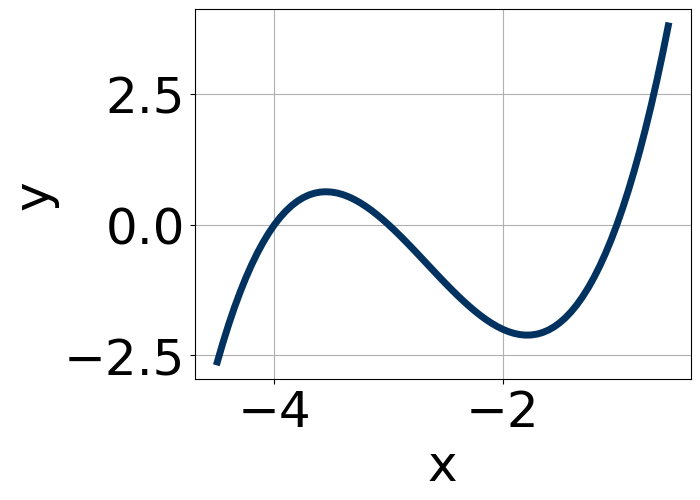
\includegraphics[width=0.5\textwidth]{../Figures/polyGraphToFunctionB.png}
\end{center}
\begin{enumerate}[label=\Alph*.]
\item \( -4x^{7} (x - 3)^{4} (x - 2)^{6} \)
\item \( 14x^{11} (x - 3)^{8} (x - 2)^{11} \)
\item \( -7x^{5} (x - 3)^{5} (x - 2)^{10} \)
\item \( -20x^{7} (x - 3)^{4} (x - 2)^{11} \)
\item \( 16x^{8} (x - 3)^{6} (x - 2)^{9} \)

\end{enumerate} }
\litem{
Describe the end behavior of the polynomial below.\[ f(x) = 6(x + 5)^{5}(x - 5)^{8}(x + 9)^{4}(x - 9)^{5} \]\begin{enumerate}[label=\Alph*.]
\begin{multicols}{2}\item 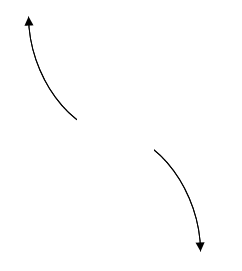
\includegraphics[width = 0.3\textwidth]{../Figures/polyEndBehaviorCopyAB.png}\item 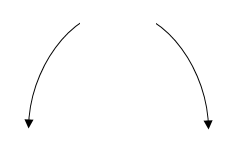
\includegraphics[width = 0.3\textwidth]{../Figures/polyEndBehaviorCopyBB.png}\item 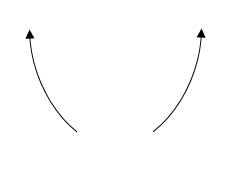
\includegraphics[width = 0.3\textwidth]{../Figures/polyEndBehaviorCopyCB.png}\item 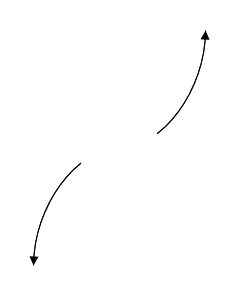
\includegraphics[width = 0.3\textwidth]{../Figures/polyEndBehaviorCopyDB.png}\end{multicols}\item None of the above.
\end{enumerate} }
\litem{
Construct the lowest-degree polynomial given the zeros below. Then, choose the intervals that contain the coefficients of the polynomial in the form $ax^3+bx^2+cx+d$.\[ \frac{-7}{5}, -3, \text{ and } 6 \]\begin{enumerate}[label=\Alph*.]
\item \( a \in [3, 6], b \in [-55, -49], c \in [153, 155], \text{ and } d \in [-130, -115] \)
\item \( a \in [3, 6], b \in [4, 14], c \in [-114, -110], \text{ and } d \in [124, 127] \)
\item \( a \in [3, 6], b \in [-11, -4], c \in [-114, -110], \text{ and } d \in [124, 127] \)
\item \( a \in [3, 6], b \in [-11, -4], c \in [-114, -110], \text{ and } d \in [-130, -115] \)
\item \( a \in [3, 6], b \in [-25, -18], c \in [-72, -66], \text{ and } d \in [124, 127] \)

\end{enumerate} }
\litem{
Which of the following equations \textit{could} be of the graph presented below?
\begin{center}
    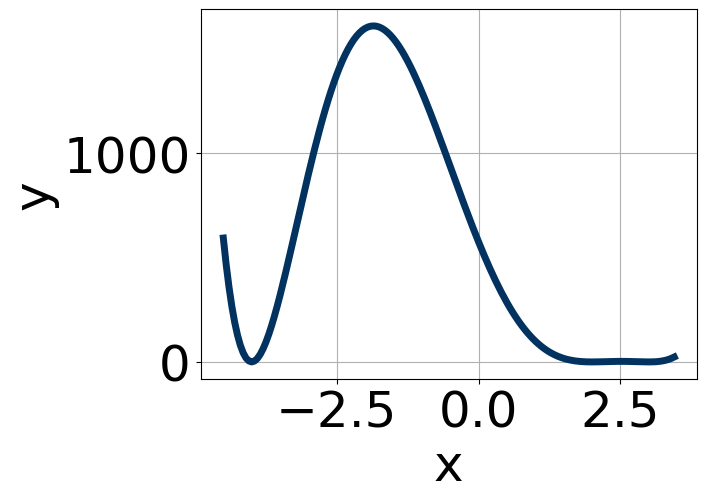
\includegraphics[width=0.5\textwidth]{../Figures/polyGraphToFunctionCopyB.png}
\end{center}
\begin{enumerate}[label=\Alph*.]
\item \( 15(x - 3)^{4} (x + 3)^{10} (x + 4)^{11} \)
\item \( -19(x - 3)^{6} (x + 3)^{9} (x + 4)^{9} \)
\item \( 15(x - 3)^{6} (x + 3)^{9} (x + 4)^{7} \)
\item \( 2(x - 3)^{7} (x + 3)^{9} (x + 4)^{7} \)
\item \( -10(x - 3)^{7} (x + 3)^{11} (x + 4)^{11} \)

\end{enumerate} }
\litem{
Describe the zero behavior of the zero $x = 5$ of the polynomial below.\[ f(x) = 4(x + 5)^{5}(x - 5)^{8}(x - 2)^{4}(x + 2)^{8} \]\begin{enumerate}[label=\Alph*.]
\begin{multicols}{2}\item 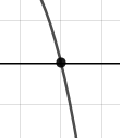
\includegraphics[width = 0.3\textwidth]{../Figures/polyZeroBehaviorAB.png}\item 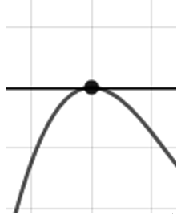
\includegraphics[width = 0.3\textwidth]{../Figures/polyZeroBehaviorBB.png}\item 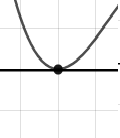
\includegraphics[width = 0.3\textwidth]{../Figures/polyZeroBehaviorCB.png}\item 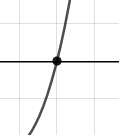
\includegraphics[width = 0.3\textwidth]{../Figures/polyZeroBehaviorDB.png}\end{multicols}\item None of the above.
\end{enumerate} }
\litem{
Construct the lowest-degree polynomial given the zeros below. Then, choose the intervals that contain the coefficients of the polynomial in the form $x^3+bx^2+cx+d$.\[ 5 - 3 i \text{ and } -2 \]\begin{enumerate}[label=\Alph*.]
\item \( b \in [0, 5], c \in [-4, 2], \text{ and } d \in [-16, -1] \)
\item \( b \in [6, 12], c \in [8, 22], \text{ and } d \in [-76, -63] \)
\item \( b \in [-8, -4], c \in [8, 22], \text{ and } d \in [63, 75] \)
\item \( b \in [0, 5], c \in [4, 13], \text{ and } d \in [-1, 10] \)
\item \( \text{None of the above.} \)

\end{enumerate} }
\litem{
Describe the zero behavior of the zero $x = 9$ of the polynomial below.\[ f(x) = -5(x + 9)^{2}(x - 9)^{3}(x - 8)^{2}(x + 8)^{5} \]\begin{enumerate}[label=\Alph*.]
\begin{multicols}{2}\item 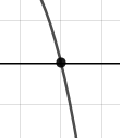
\includegraphics[width = 0.3\textwidth]{../Figures/polyZeroBehaviorCopyAB.png}\item 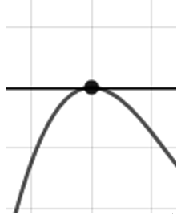
\includegraphics[width = 0.3\textwidth]{../Figures/polyZeroBehaviorCopyBB.png}\item 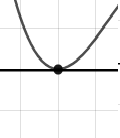
\includegraphics[width = 0.3\textwidth]{../Figures/polyZeroBehaviorCopyCB.png}\item 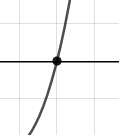
\includegraphics[width = 0.3\textwidth]{../Figures/polyZeroBehaviorCopyDB.png}\end{multicols}\item None of the above.
\end{enumerate} }
\litem{
Describe the end behavior of the polynomial below.\[ f(x) = 8(x + 2)^{5}(x - 2)^{8}(x + 3)^{2}(x - 3)^{2} \]\begin{enumerate}[label=\Alph*.]
\begin{multicols}{2}\item 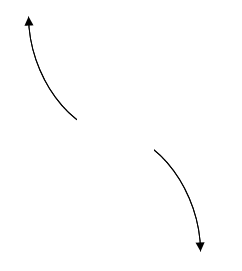
\includegraphics[width = 0.3\textwidth]{../Figures/polyEndBehaviorAB.png}\item 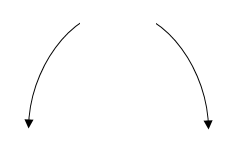
\includegraphics[width = 0.3\textwidth]{../Figures/polyEndBehaviorBB.png}\item 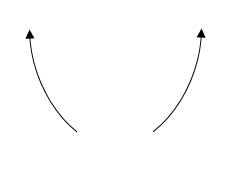
\includegraphics[width = 0.3\textwidth]{../Figures/polyEndBehaviorCB.png}\item 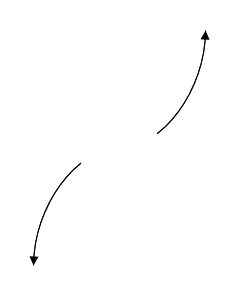
\includegraphics[width = 0.3\textwidth]{../Figures/polyEndBehaviorDB.png}\end{multicols}\item None of the above.
\end{enumerate} }
\end{enumerate}

\end{document}